% ====== TAREA 1 MATEMATICAS APLICADAS ======

\documentclass{article}
\usepackage[utf8x]{inputenc}
\usepackage[spanish]{babel}
\usepackage{cancel}
\usepackage{amsmath}
\usepackage{amsfonts}
\usepackage{amssymb}
\usepackage{graphicx}
\usepackage{enumitem}
\usepackage[text={20cm,25cm},centering,top=1.5cm,bottom=1.5cm,letterpaper,showframe=false]{geometry}
\renewcommand{\baselinestretch}{1.5}
\parindent  = 0mm
\parskip    = 4mm

\begin{document}
\title{Tarea 1}
        \author{Careaga Carrillo Juan Manuel \\ Quiróz Castañeda Edgar \\ Soto Corderi Sandra del Mar}
        \date{Lunes 21 de Septiembre del 2018}
        \maketitle

	\begin{enumerate}
   	% Ejercicio 1
   	\item {
   Dibujar la región W definida por las superficies $x + 2y + 3z = 6$ y $z = 0$. Expresar la integral triple $\iiint_Wf(x,y,z)dV$ de las seis formas posibles como integrales iteradas.\\

	}

	% Ejercicio 2
   \item {
    Dibujar la región W descrita por la integral iterada
    \begin{center}
    $\int_{0}^{1}\int_{z^3}^{\sqrt{z}}\int_{0}^{4-x}dydxdz$. 
    \end{center}
    Calcular su volumen.\\
		     
	}


	% Ejercicio 3
   \item {
    Integrar la función $f(x,y) = x^2 + 2xy^2 + 2$ sobre la región $D$ acotada por la gráfica de $y = -x^2 + x$, el eje $x$, y las rectas $x = 0$ y $x = 2$.\\


	}

	% Ejercicio 4
    \item {
        Usar integrales dobles para calcular el área de una elipse con semiejes $a$ y $b$.

        Supongamos, sin perder la generalidad, que $a\geq b$. La ecuación canónica de la elipse horizontal cuyo centro está en el origen del plano y tiene semiejes $a$ y $b$ es
        \[
            \frac{x^2}{a^2}+\frac{y^2}{b^2}=1
        \]
        Equivalentemente, podemos afirmar entonces que
        \(\displaystyle
            y=\frac{\pm\sqrt{a^2 b^2 -b^2 x^2}}{a}
        \)
        describe nuestro lugar geométrico. Por simplieza, y aprovechando su simetría con los ejes $X$ e $Y$, dividimos la elipse en 4 regiones iguales delimitadas por los ejes coordenados y únicamente calcularemos el área de una de ellas, llámese $R$, al final, el área total se obtendrá de multiplicar el área de dicha región por 4.
        \begin{center}
            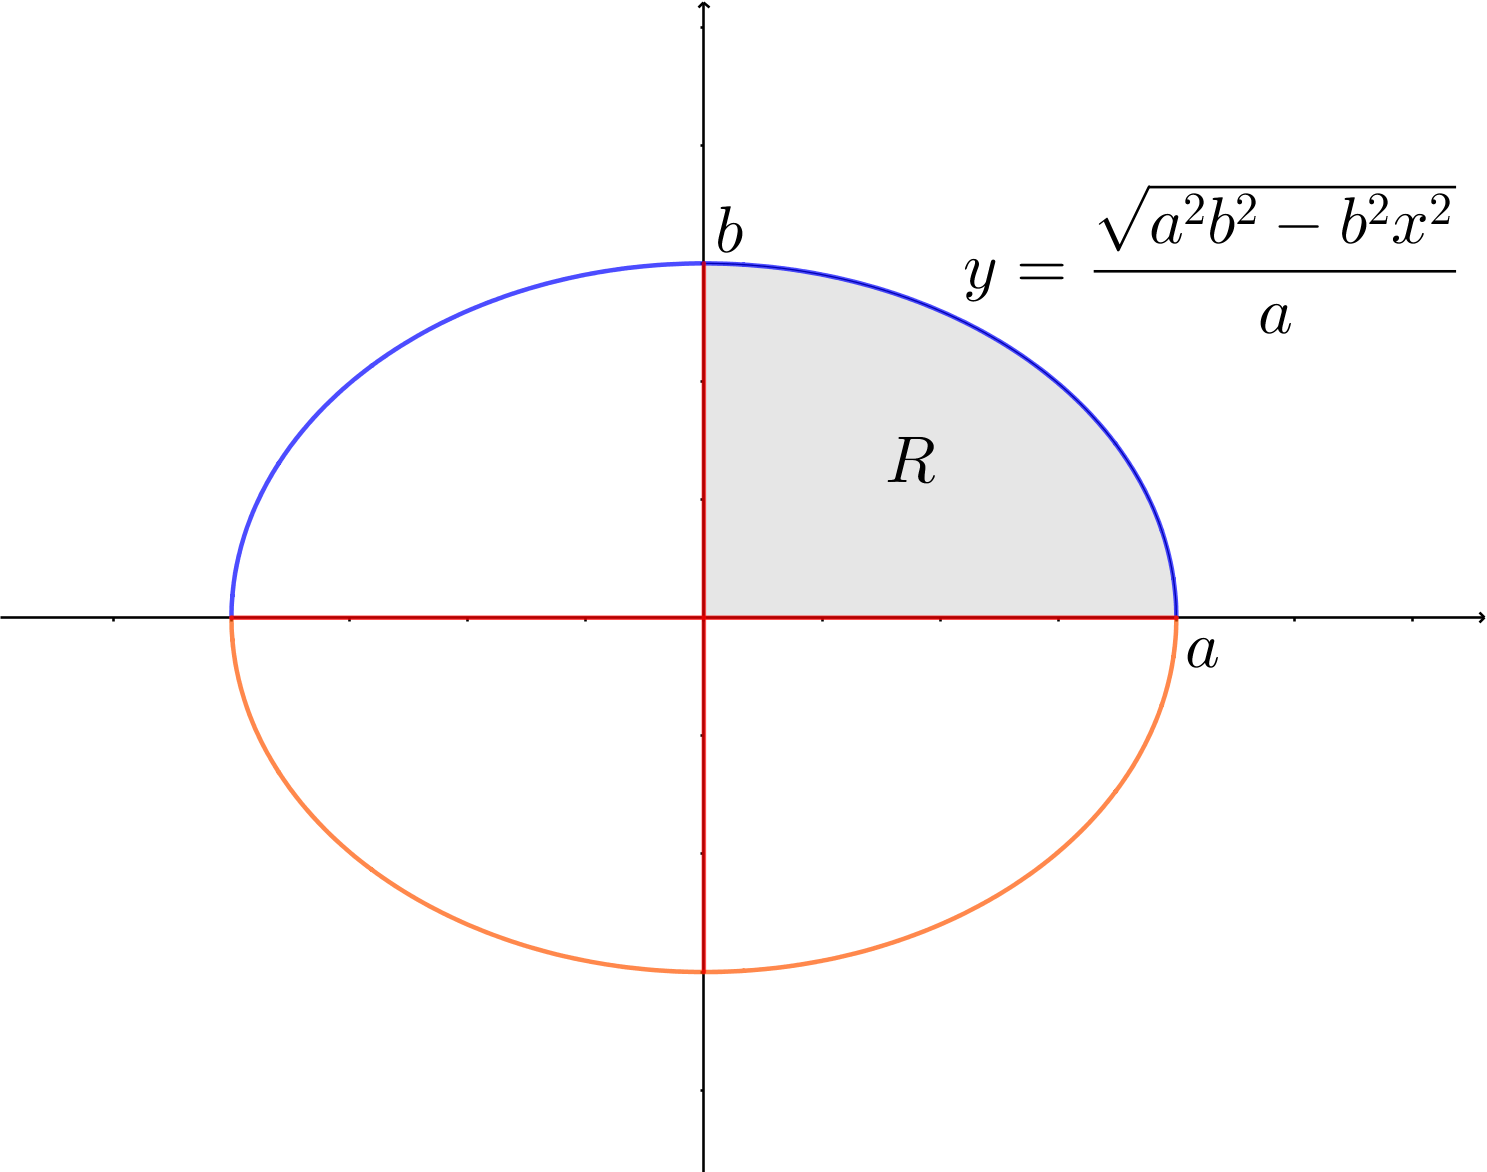
\includegraphics[width=6cm]{img/ej4.png}
        \end{center}
        $R$ es una región $y-$simple, por lo que
        \(\displaystyle
            R=\left\{
                (x,y)\,\bigg\vert\,
                0\leq x\leq a;
                0\leq y\leq\frac{\sqrt{a^2b^2-b^2x^2}}{a}
            \right\}
        \)
        , entonces el área de $R$ está dada por
        \[
            \iint_R{dA}
            =\int_0^a{\int_0^{ \frac{\sqrt{a^2b^2-b^2x^2}}{a} }{dy}\,dx}
            =\int_0^a{\frac{1}{a}\sqrt{a^2b^2-b^2x^2}\,dx}
            =\frac{b}{a}\int_0^a{\sqrt{a^2-x^2}\,dx}
        \]
        Haciendo la sustitución $x=a \sen{\theta}$ con $0\leq\theta\leq\frac{\pi}{2}$, tenemos que $dx=a\cos{\theta}\,d\theta$; para los límites de la integral, si $x=0=a\sen{\theta}$ entonces $\theta=0$ y si $x=a=a\sen{\theta}$, entonces $\theta=\frac{\pi}{2}$. La integral queda como
        \[
            \frac{b}{\cancel{a}}\int_0^{\frac{\pi}{2}}{
                \sqrt{a^2-a^2\sen^2{\theta}}\,\cancel{a}\cos{\theta}\,d\theta
            }
            =b\int_0^{\frac{\pi}{2}}{
                \sqrt{a^2(1-\sen^2{\theta})}\cos{\theta}\,d\theta
            }
            =ab\int_0^{\frac{\pi}{2}}{
                \cos^2{\theta}\,d\theta
            }
        \]
        Usando la fórmula del ángulo doble para el coseno tenemos
        \[
            =ab\int_0^\frac{\pi}{2}{
                \frac{1}{2}(1+\cos{(2\theta)})
            \,d\theta}
            =\frac{ab}{2}\left[
                \theta + \frac{1}{2}\sen{(2\theta)}
            \right]_0^\frac{\pi}{2}
            =\frac{ab}{2}\left[
                \frac{\pi}{2}+0
            \right]
            =\frac{\pi ab}{4}
        \]
        Por lo tanto, el área de la elipse es 4 veces lo anterior, es decir $A=\pi ab$
	}

	% Ejercicio 5
    \item {
        Mostrar que al evaluar $\iint_DdA$, donde $D$ es una región $y$-simple, se reproduce la fórmula del cálculo de una variable para el área entre dos curvas.

        Sea $D$ una región $y-$simple, entonces de define como
        \(
            D=\left\{
                (x,y)\,\bigg\vert\, a\leq x\leq b;\;
                \varphi_1(x)\leq y\leq\varphi_2(x)
            \right\}
        \)
        para algunos $a,b\in\mathbb{R}$ y $\varphi_1(x):\mathbb{R}\rightarrow\mathbb{R}$, $\varphi_2(x):\mathbb{R}\rightarrow\mathbb{R}$. Entonces
        \[
            \iint_D{dA}
            =\int_a^b{
                \int_{\varphi_1(x)}^{\varphi_2(x)}{dy}
            \,dx}
        \]
        por el Teorema de Fubini
        \[
            =\int_a^b{
                \left[ y \right]_{\varphi_1(x)}^{\varphi_2(x)}
            \,dx}
            =\int_a^b{
                \left[ \varphi_2(x) - \varphi_1(x) \right]
            \,dx}
            =\int_a^b{\varphi_2(x)\,dx}
            -\int_a^b{\varphi_1(x)\,dx}
        \]
        que es como se calcula el área comprendida entre las curvas $\varphi_1(x)$ y $\varphi_2(x)$ en el intervalo $[a,b]$.
    }

	% Ejercicio 6
   \item {
   Describir la región que se encuentra entre el cono $z = \sqrt{x^2 + y^2}$ como una región elemental.\\

	
    }
    
    % Ejercicio 7
   \item {
   Hallar el volumen acotado por el paraboloide $z = 2x^2 + y^2$ y el cilindro $z = 4 - y^2$\\

	
    }
    
    % Ejercicio 8
   \item {
    \begin{enumerate}
	\item
	Investigar qué es el centro de masa de un cuerpo y cómo se puede calcular usando integrales múltiples.\\	
	
	
	\item    
	La densidad en un punto $P$ de un cubo sólido de lado $a$ es directamente proporcional al cuadrado de la distancia del punto $P$ a una esquina fija del cubo. Encontrar el centro de masa.\\    
    
    \end{enumerate}
    }
    
\end{enumerate}
\end{document}
